\item \subquestionpoints{5}
Investigate why the training procedure behaves unexpectedly on dataset $B$, but
not on $A$. Provide hard evidence (in the form of math, code, plots, etc.) to
corroborate your hypothesis for the misbehavior. Remember, you should address
why your explanation does \emph{not} apply to $A$.

\textbf{Hint}: The issue is not a numerical rounding or over/underflow error.

\ifnum\solutions=1 {
  
\begin{answer}

\begin{figure}[htbp]
\begin{subfigure}[b]{0.5\linewidth}
    \centering
    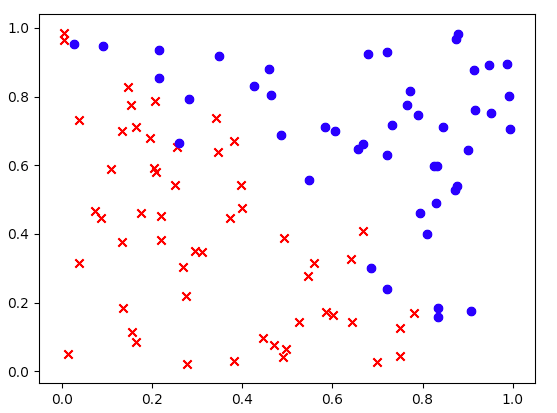
\includegraphics[width=\linewidth]{pics/F1b-b.png}
    \caption{Dataset A}\label{fig:dataset-a}
\end{subfigure}
\begin{subfigure}[b]{0.5\linewidth}
    \centering
    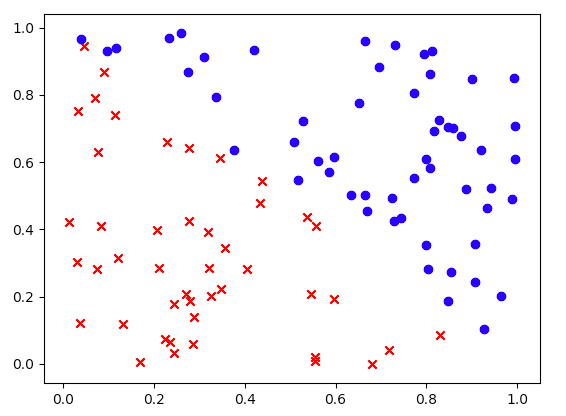
\includegraphics[width=\linewidth]{pics/F1b-a.png}
    \caption{Dataset B}\label{fig:dataset-b}
\end{subfigure}
\caption{Datasets}
\label{fig:datasets}
\end{figure}

Figure~\subref{fig:dataset-a} and Figure~\subref{fig:dataset-b} shows the two datasets. The problem is that dataset B is perfectly linearly separable. 

Consider optimizing objective:

$$
    L(\theta) = \prod_{i=1}^mp(y^{(i)}|x^{(i)};\theta) = \frac{1}{1 + e^{-y^{(i)}\theta^T x^{(i)}}}
$$

    Since the algorithm tries to find the maximum likelihood. if the data is linearly separable(i.e. all $y^{(i)}\theta^T x^{(i)}$ can be positive), every $ \frac{1}{1 + e^{-y^{(i)}\theta^T x^{(i)}}} $ can be small by augmenting the norm of $ \theta $ so after perfectly separate them the algorithm tends to augment $ \theta $ to infinity.
    
    If the data isn't linearly separable(i.e.  $\exists\  y^{(i)}\theta^T x^{(i)}$ to be negative), in this case, the algorithm cannot augment $ \theta $ infinitely since the negative $y^{(i)}\theta^T x^{(i)}$ constraints $ \frac{1}{1 + e^{-y^{(i)}\theta^T x^{(i)}}} $  to be very small while $ \|\theta\| $ is large. just like the regularization term. So there is a trade-off while maximizing the likelihood. 
\end{answer}


} \fi
